\section{Задача 2.7}
\subsection{Задание:}
При каких условиях модуль суммы двух комплексных чисел равен разности модулей слагаемых?
\subsection{Решение:}
$
	z_1 = x_1 + i y_1\\
	z_2 = x_2 + i y_2\\
$
Модуль суммы $ z_1 $ и $ z_2 $ это длинна вектора, составленного как векторная сумма $ z_1 $ и $ z_2 $.\\
Таким образом модуль суммы двух комплексных чисел будет равен разности модулей слагаемых когда векторы,
соответствующие $ z_1 $ и $ z_2 $ на плоскости комплексных чисел будут противоположно направленными, то есть
должно выполняться условие:
\\[1em]
$
	\dfrac{x_1}{x_2} = \dfrac{y_1}{y_2} < 0
$
\subsection{Компьютерная проверка в среде Wolfram Mathematica}
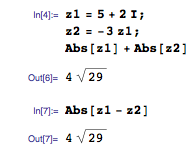
\includegraphics[scale=0.6]{task/2_07/screen1.png}
\subsection{Вывод:}
Мы нашли условие при котором модуль суммы двух комплексных чисел равен разности модулей слагаемых.
